\documentclass[sigconf]{acmart}
\renewcommand\footnotetextcopyrightpermission[1]{}
\usepackage{csquotes}

%%für Deutsch
\usepackage[utf8]{inputenc}
\usepackage[T1]{fontenc}
\usepackage[ngerman]{babel}  % Fügt das Babel-Paket für deutsche Sprache hinzu

\usepackage{graphicx}
\bibliographystyle{plain}
\title{The Devil is in the Detail: Issues with Fine-Grained Trusted Execution Environments}
\author{Jonathan Adshead}
\email{jonathan.adshead@fau.de}
\affiliation{
    \institution{Friedricht-Alexander-Universität Erlangen-Nürnberg}
    \country{}}
\makeatletter

\let\@authorsaddresses\@empty 
\makeatother
\pagestyle{plain}
\settopmatter{printacmref=false}
\settopmatter{printfolios=false}

\acmConference[FAU]{Make sure to enter the correct
  conference title from your rights confirmation emai}{Mai 2024}{Erlangen, Deutschland}

\setlength{\parindent}{0pt} %%stoppt die Einrückung

\begin{document}

\maketitle  % Dieser Befehl erzeugt den Titel, Autor und Datum im Dokument


%%Für die Seitennummerierung
%%\thispagestyle{plain} %%damit auch die erste seite eine 1 hat
%%\pagenumbering{arabic}
%%\pagestyle{plain} %%???

%%\renewcommand{\shortauthors}{Trovato et al.}


\section*{Kurzfassung}
Mit dem Aufstieg des Cloud-Computing und der zunehmenden Verlagerung sensibler Daten und kritischer Anwendungen in die Cloud gewinnen Trusted Execution Environments (TEEs) an Bedeutung. Das Hauptziel von TEEs ist die Minimierung der Angriffsfläche und die Isolation von Schwachstellen, um die Integrität und Vertraulichkeit der Daten zu gewährleisten. TEEs bieten eine geschützte Umgebung zur sicheren Verarbeitung und Speicherung sensibler Daten, sind jedoch nicht frei von Schwachstellen. 
Dieses Paper untersucht die Sicherheitslücken feingranularer TEEs und kategorisiert diese in zwei Hauptkategorien: Datenlecks und Datenkorruption. Es wird gezeigt, dass die Schnittstellen zwischen verschiedenen TEEs sowie zwischen sicheren Anwendungen in einer TEE und unsicheren Anwendungen zu erheblichen Sicherheitsrisiken führen können.
Die Ziele dieser Arbeit sind die Darstellung von potenziellen Angriffen und Auswirkungen dieser, um die Sicherheit und Isolation von TEEs zu verbessern. Die Arbeit stützt sich auf die Studien \enquote{Assessing the Impact of Interface Vulnerabilities in Compartmentalized SoftwareAssessing the Impact of Interface Vulnerabilities in Compartmentalized Software}~\cite{CIVPaper} und \enquote{Assessing the Impact of Interface Vulnerabilities in Compartmentalized Software}~\cite{TEEPaper}.

\section{Einleitung}
Die zunehmende Entwicklung im Bereich des Cloud-Computing und Verbreitung von Cloud-Diensten haben die Nachfrage von verteilten Computersystemen stark erhöht. 
Immer mehr Unternehmen und Organisationen verlagern Teile oder ihre gesamten Anwendungen in die Cloud, mit der Erwartung, von Skalierbarkeit, Flexibilität und Kosteneffizienz zu profitieren~\cite{Cloud}. 
Mit der Nutzung sensibler Daten und kritischer Anwendungen gewinnt die Sicherheit dieser Cloud-Infrastrukturen an Bedeutung, da sie potentiell die sensiblen Informationen von Millionen von Nutzern und Organisationen verwalten.

TEEs sind dadurch zu einer wichtigen Technologie geworden, um die Sicherheit sensibler Daten und kritischer Anwendungen in einer geschützen Umgebung zu gewährleisten. Doch trotz ihrer wichtigen Rolle sind TEEs nicht frei von Schwachstellen. 

Das Grundprinzip der TEEs erzwingt eine duale Weltansicht in den Hardwarekomponenten, welche in eine (1) normale, möglicherweise kompromittierte und eine (2) sichere und isolierte Welt aufgeteilt ist~\cite{TEEPaper}. 
Dabei können kompromittierte oder bösartige Systemsoftwareteile in der normalen, bzw. kompromittierten Welt keine Daten auf dem sicheren Speicherbereich der Enklave, welche einen isolierten Bereich im Adressraum bezeichnet, lesen. In Abschnitt 2.1 wird näher auf Enklaven eingegangen. Vor allem diese, durch die duale Weltansicht entstehende Schnittstelle zwischen verschiedenen TEEs und zwischen TEE und Programmen in der unsicheren Welt, stellen einen potenziellen Angriffsvektor dar.
Diese Schwachstelle birgt das Risiko von Datenlecks und Datenkorruption, sowie Seitenkanalangriffen oder Rollback-Angriffen~\cite{Memory, TEEPaper}. Ein erfolgreiches Ausnutzen dieser Schwachstellen von Angreifern kann nicht nur sensible Informationen kompromittieren, sondern auch die Integrität der gesamten Enklave gefährden. 

Dieses Paper legt den Fokus auf die Sicherheitslücken, sowohl zwischen den unterschiedlichen TEEs als auch zwischen sicheren Anwendungen einer TEE und Anwendungen der unsicheren Welt. Der Fokus liegt dabei auf Angriffen, die zu Datenlecks und Datenkorruption führen können.

\section{Grundlagen}
Die Trusted Execution Environment (TEE) zeichnet sich durch drei wesentliche Eigenschaften aus, die ihre Funktionalität und Sicherheit beschreiben. Sie gewährleistet (1) die Authentizität des ausgeführten Codes, indem sie sicherstellt, dass dieser tatsächlich von der beabsichtigten Quelle stammt und nicht manipuliert wurde.  Sie sichert (2) die Integrität des Codes, indem sie während der Ausführung sicherstellt, dass dieser nicht verändert wurde und sie schützt (3) die Vertraulichkeit von Code, Daten und Laufzeitvariablen, indem sie sicherstellt, dass diese nur von privilegierten Parteien eingesehen werden kann. 

Aufgrund der Interaktion von Programmen innerhalb der TEE und Programmen außerhalb, kann die TEE auch als Kompartiment betrachtet werden. Diese Struktur ermöglicht eine klare Trennung zwischen den unterschiedlichen Kompartiments und ermöglicht so eine bessere Kontrolle über den Zugriff.

\subsection{TEE}
Der genaue Aufbau und das Verhalten von Trusted Execution Environments (TEEs) variieren, lassen sich aber im Allgemeinen in zwei Kategorien einteilen: (1) TEEs, die sich einen Adressraum mit dem unprivilegierten Host teilen, und (2) TEEs, bei denen die CPU konzeptionell in eine normale und eine sichere Welt unterteilt ist.

In der ersten Kategorie hat nur die Enklave selbst vollen Zugriff auf ihren Speicherplatz und kann die Daten im Klartext lesen. Eine Enklave ist ein isolierter Speicherbereich innerhalb einer TEE, der dazu dient, Code und Daten vor unautorisiertem Zugriff und Manipulation zu schützen. Selbst privilegierte Benutzer und das Betriebssystem haben keinen Zugriff auf die innerhalb der Enklave gespeicherten Daten. Programme innerhalb der Enklave dürfen jedoch auch auf den Adressraum außerhalb der Enklave zugreifen.Diese Struktur ermöglicht einen besseren Datenaustausch, birgt jedoch das Risiko unsicherer Speicherzugriffe, was potenziell zu Sicherheitslücken führen kann.

In der zweiten Kategorie ist der Adressraum strikt in zwei separate Bereiche unterteilt, wobei keiner der beiden Bereiche auf den jeweils anderen zugreifen kann. Der Datenaustausch zwischen diesen beiden Welten erfolgt über das Trusted Operating System (TOS). Da das TOS privilegierten Zugriff hat, kann es einen geteilten Adressraum einrichten, in dem Daten sicher ausgetauscht werden können. Diese Methode bietet eine stärkere Isolation und somit ein höheres Maß an Sicherheit, da direkte Speicherzugriffe zwischen der normalen und der sicheren Welt verhindert werden, jedoch auf Kosten der Datenübertragungsraten.

In beiden Kategorien gewährleistet sowohl der Prozessor, dass extern kein Zugriff auf die Daten möglich ist, als auch das TOS, dass der Code in der Enklave sicher ist. Ein weiterer Grundgedanke beim Designen einer TEE ist Angreifermodel. Man entwickelt die TEE unter der Annahme, dass sie in einem System ausgeführt wird, das als kompromittiert betrachtet wird und Angreifer die volle Kontrolle über sämtliche Hardware haben.

Das TOS übernimmt den Entry/Exit Prozess der TEE, in dem der Übergang zwischen der normalen und der sicheren Welt ausgeführt wird. Dabei müssen die Daten, wie die Register flags oder der Call stack, aber auch die Eingabedaten, bereinigt werden. Im Exit prozess müssen wiederum die Daten bereinigt werden, damit sie nicht ausgelesen werden können.

Neben den Angriffen auf der Application Binary Interface (ABI), welche auf Schwachstellen beim erstellen und verlassen der TEE abzielen, gibt es noch die Apication Programming Interface, welche versuchen Sicherheitslücken während der Laufzeit zu nutzen.
\subsection{Kompartimentierung}

Die Kompartimentierung ist ein Konzept, das darauf abzielt, ein Computersystem oder einzelne Anwendungen in separate Bereiche aufzuteilen und diese möglichst isoliert voneinander operieren zu lassen. Diese Praxis beruht auf den Prinzipien der Sandbox und der Safebox, die eine sicherere und stabilere Systemumgebung ermöglichen. 

Eine Sandbox ist eine isolierte Ausführungsumgebung, in dem ein Programm ausgeführt wird, welches keinen Zugriff auf Daten anderer Programme hat. Dies gewährleistet nicht nur die Sicherheit sensibler Informationen, sondern verhindert auch die Übernahme von Daten oder die Beeinflussung des Programmes durch potenziell kompromittierte Softwareteile.


Im Gegensatz dazu dient die Safebox dem Schutz der eignen Daten. Dies wird ermöglicht, indem nur privilegierten Prozessen Zugriff auf die Daten gestattet wird. Diese Zugangskontrolle verhindert den Zugriff auf Daten eines anderen Kompartiments. 

Die Kombination aus Sandboxing und Safeboxing ermöglicht eine Trennung zwischen den einzelnen Teilen eines Programmes und sorgt so dafür, dass eine Übernahme des Systems oder ein Zugang zu vertraulichen Daten erschwert wird.

Das Initialisieren eines Kompartments lässt sich in 3 Stufen unterteilen. Zunächst erfolgt die Identifizierung, wo das Programm logisch gut unterteilt werden kann und wie feingranular diese Unterteilung sein soll. Anschließend wird die Durchsetzung der Grenzen vorgenommen, indem die Programme logisch voneinander getrennt und ausschließlich über eine API zur Kommunikation zugelassen werden. 

In der letzten Stufe werden diese Grenzen weiter verstärkt. Hierbei werden die API-Schnittstellen klarer definiert, der Datenfluss möglichst reduziert und Strategien implementiert, wie mit potenziell unsicheren Daten von der unsicheren Welt umgegangen wird.

\begin{figure}[h]
    \centering
    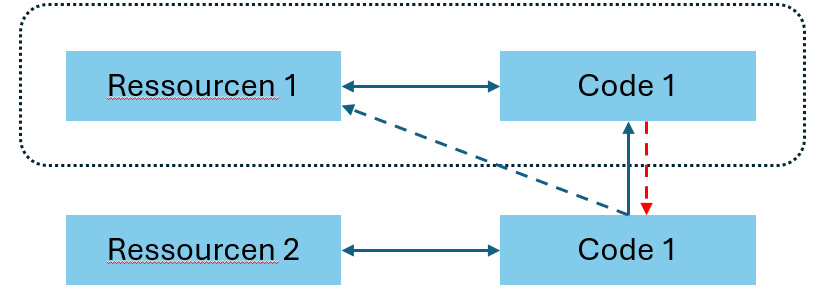
\includegraphics[width=\linewidth]{Grafiken/Sandbox.png}
    \caption{Beschreibung deiner Abbildung hier.}
    \label{fig:sandbox}
\end{figure}
\begin{figure}[h]
    \centering
    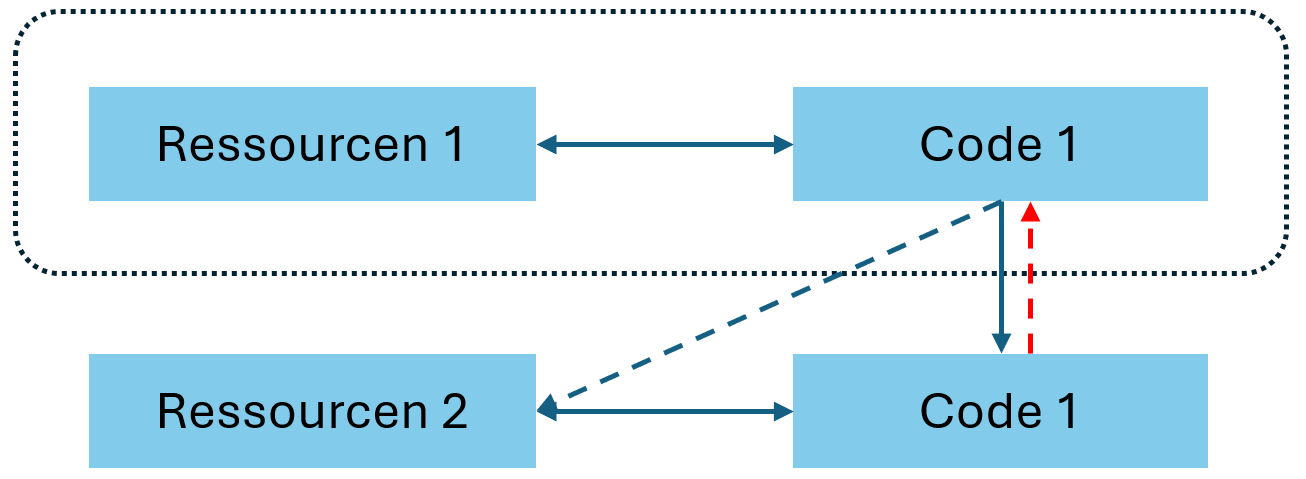
\includegraphics[width=\linewidth]{Grafiken/Safebox.png}
    \caption{Beschreibung deiner Abbildung hier.}
    \label{fig:Safebox}
\end{figure}
\begin{figure}[h]
    \centering
    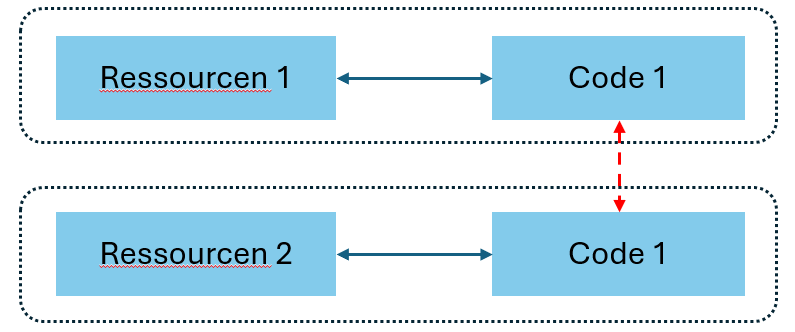
\includegraphics[width=\linewidth]{Grafiken/Kompartiment.png}
    \caption{Beschreibung deiner Abbildung hier.}
    \label{fig:Kompartment}
\end{figure}



\section{Ziele von feingranularen TEEs}
Ein wichtiger Begriff im Zusammenhang von TEEs ist die Trusted Computing Base (TCB). Die TCB beschreibt den Bereich eines Programms, der besonders vor externen Angriffen geschützt werden muss, da er mit sensiblen Daten arbeitet oder andere kritische Funktionen übernimmt, wie z. B. das Interagieren mit sensiblen Daten. Wird nun ausschließlich dieser Teil der Anwendung in einer TEE ausgeführt, wird von einer feingranularen TEE gesprochen.

Außerdem können mehrere feingranulare TEEs genutzt werden, indem mehrere kritische Funktionen in separaten TEEs ausgeführt werden, was die Sicherheit weiter erhöhen kann.

\subsection{Minimierung der Angriffsfläche}
Das Hauptziel für die Verwendung von feingranularen TEEs ist die Minimierung der Angriffsfläche und damit die Erhöhung der Sicherheit, die sie liefert. 

Programme aus der unsicheren Umgebung haben keinen direkten Zugriff auf Daten, die innerhalb der sicheren Enklave verarbeitet werden. Da feingranulare TEEs in diesem Kontext als Kompartimente behandelt werden können, gibt es für die Kommunikation zwischen sicherer und unsicherer Welt eine definierte Schnittstelle, auch als Enklave Description Language (EDL) bekannt. 

Diese Schnittstelle ermöglicht es, genau zu kontrollieren, welche Daten und in welchem Format diese Daten von außen akzeptiert werden. Obwohl diese Schnittstelle die Sicherheit erhöht, stellt sie dafür einen neuen Angriffsvektor dar und führt zu einer neuen Klasse von Sicherheitsproblemen, den Compartment Interface Vulnerabilities (CIVs) \cite{CIVPaper}.

\subsection{Isolierung von Schwachstellen}
Ein weiteres wichtiges Ziel feingranularer TEEs ist ihre Fähigkeit zur Isolierung von Schwachstellen. Ziel ist es, die Kompartimente sicherer zu machen und in der Zukunft die Unabhängigkeit der Kompartimente voneinander zu erreichen.


Es wird immer weiter darauf hingearbeitet, dass Sicherheitslücken in einem Kompartiment keine Auswirkungen auf die anderen Kompartimente haben und so eine Isolation der Sicherheitslücken entsteht. Je mehr Kompartimente eingesetzt werden, desto widerstandsfähiger wird das gesamte System gegen Angriffe. Allerdings steigt mit der Anzahl der feingranularen TEEs auch der Aufwand für die Erstellung, Überprüfung und Verwaltung der Daten sowie der gesamte Overhead. Dennoch kann ein erfolgreicher Angriff auf ein einzelnes Kompartiment möglicherweise nur einen Teil der Daten kompromittieren, während der Rest des Systems sicher bleibt.


\section{Sicherheitsprobleme von feingranularen TEEs}
Wird die Sicherheit der Daten betrachtet, offenbart sich ein signifikanter Unterschied zwischen TEEs mit einem gemeinsamen Adressraum und solchen mit einem separaten. 
Bei streng separierten Enklaven gestaltet es sich äußerst schwierig für unsichere Prozesse, die TEE zur Freigabe von Daten aus ihrem Speicher zu bringen.
Die Konfiguration des TOS kann entweder eine Spiegelung eines Teils des Adressraums oder den Zugriff auf externe Daten für den Datenaustausch in und aus der Enklave ermöglichen. 
In beiden Fällen ist jedoch kein direkter Zugriff des Programms auf den Speicher der Anwendung möglich.

Hugo Lefeuvre et al.~\cite{CIVPaper} haben zwei große Kategorien von Sicherheitslücken identifiziert: Datenlecks und Datenkorruption. Diese Kategorisierung erweist sich als nützlich, da nahezu alle bekannten Angriffe auf TEEs in eine dieser beiden Kategorien fallen. Auch die Angriffsvektoren, die von Jo Van Bulck et al.\cite{TEEPaper} gefunden und untersucht wurden, lassen sich in diese Kategorien einteilen, was die Gültigkeit dieser Klassifizierung weiter unterstützt. Die Einteilung in Datenlecks und Datenkorruption ermöglicht eine Identifizierung der Angriffsziele und eine Einschätzung der potenziellen Auswirkungen auf die Sicherheit und Integrität der Daten.

\subsection{Datenlecks}
Die Kategorie der Datenlecks umfasst Angriffe, die darauf abzielen, Daten aus der Enklave zu extrahieren. 

\subsubsection{Angriff beim Erstellen und Verlassen}
Ein besonders anfälliges Angriffsziel ist der Zustand der TEE beim Verlassen oder Beenden. Unabhängig davon, ob die Beendigung geplant oder durch ein Interrupt erzwungen wird, muss sichergestellt werden, dass keine Daten in einem lesbaren Zustand im Speicher verbleiben. Da das Bereinigen des Speichers eine explizite Softwareaufgabe darstellt, liegt es in der Verantwortung der Entwickler, dies korrekt zu implementieren. Selbst wenn das Bereinigen der Registerzustände in normalen Prozesswechseln üblich ist und automatisch erfolgt, ist diese Schwachstelle nicht zu unterschätzen. Wird dieser Prozess nicht ordnungsgemäß durchgeführt, können Angreifer Registereinträge oder den Stack auslesen und dadurch Rückschlüsse auf die Funktionsweise der Anwendung und die letzten Aktionen innerhalb der TEE ziehen.

Die Bedeutung dieser Sicherheitsmaßnahmen wird durch die potenziellen Konsequenzen unzureichender oder fehlerhafter Speicherbereinigung verdeutlicht. Angreifer könnten sensible Informationen wie kryptografische Schlüssel, Passwörter oder andere vertrauliche Daten extrahieren und somit die Sicherheit der gesamten Anwendung kompromittieren.

\subsubsection{Angriff mithilfe von Pointern}
Neben dem Zeitpunkt des Verlassens der TEE ist diese auch während der Laufzeit angreifbar. Konkret ist das über die Parameter möglich, die die TEE von unsicheren Prozessen von außen bekommt. Es ist essenziell, diesen Parametern nicht von Anfang an zu vertrauen. Diese Daten müssen zuerst überprüft und gegebenenfalls bereinigt werden.  Beispielsweise muss überprüft werden, ob der Inputpointer und der gesamte Speicherbereich, auf den er zeigt, außerhalb der Enklave liegen, was je nach Datentyp oder Struktur nicht nur aus einer einfachen Überprüfung besteht. Da die Größe des Pointers Teil der Eingabe ist und nach dem Angreifermodell davon ausgegangen wird, dass das komplette System möglicherweise kompromittiert ist, kann diesem Wert nicht vertraut werden.

Eine mögliche Angriffsmethode besteht darin, Situationen zu erzeugen, in denen die Größe wegen Überläufen nicht mehr richtig berechnet werden kann. Dadurch wird nicht erkannt, dass der Datenbereich tatsächlich den der Enklave schneidet. Aus diesem Grund ist es dringend notwendig, beim Berechnen von Adressen und beim grundsätzlichen Verwenden von unsicheren Daten, sichere Arithmetik zu verwenden, um fehlerhafte Berechnungen zu vermeiden.

\subsubsection{Angriff mithilfe von Strings}
Dieses Angriffsszenario kann aber Mithilfe der Manipulation von Strings noch weitergeführt werden. In Low-Level-Sprachen wie C verhält sich ein String auch als Pointer, der auf ein Array zeigt, wobei die Länge angegeben werden muss. 
Gelingt es einem Angreifer, den Datenbereich mit dem der Enklave überschneiden zu lassen, kann er nahezu den gesamten Speicher auslesen. Durch die absichtlich falsche Größenangabe und das Weglassen der Nullterminierung, die das Ende eines Strings definiert, kann der Angreifer, über das Programm in der TEE auf die Daten innerhalb der Enklave zugreifen. 
Damit kann der Angreifer über diesen Seitenkanal die Daten auslesen. 
Ein Seitenkanalangriff meint dabei, dass Rückschlüsse über die Daten z. B. anhand der Ausführungszeit oder der Cache-Zugriffe gewonnen werden können. Wird nun der String ausgelesen, kann der Angreifer anhand der Dauer feststellen, wann das nächste Nullbyte im Speicher liegt. 
Wird dies nun an beliebigen oder allen Speicheradressen gemacht, können alle Nullbytes in der Enklave identifiziert werden~\cite{TEEPaper}.

Je nach Implementierung der TEE gibt es verschiedene Arten, den Angriff durchzuführen. Beispielsweise ermöglicht das Intel SGX-SDK Angreifern, ein volles Speicherabbild zu generieren. Konkret ermöglicht das EDL-Attribut, welches das Ende eines String definiert, das Auslesen von Speicherinhalten. Standardmäßig wird das Nullbyte verwendet, aber durch das Überschreiben mit anderen Werten ist es möglich, alle entsprechenden Speicherinhalte zu lokalisieren. Wird dieser Vorgang bis 255 wiederholt, kann ein vollständiges Speicherabbild erstellt werden. Die Sicherheit der TEE ist damit vollständig umgangen worden.~\cite{IntelSGX, TEEPaper}.

Bei diesem Angriff ist anzumerken, dass TEEs nach dem Single-World-Prinzip deutlich anfälliger sind, da die Enklave in den Speicher des Angreifers eingebettet ist. Bei TEEs nach dem Two-Worlds-Prinzip werden die Daten nur über das TOS geteilt. Da aber in keinem System eine absolute Sicherheit möglich ist, gibt es auch hier Schwachstellen, die von Angreifern ausgenutzt werden können.

\subsection{Datenkorruption}
Angriffe dieser Kategorie versuchen die Daten zu überschreiben, um dadurch das Verhalten der TEE zu beeinflussen oder die Integrität zu untergraben.

Eine Möglichkeit, dies zu erreichen, besteht in der Manipulation von Register Flags. Insbesondere die Alignment Check (AC) Flag und die Direction Flag (DF) beeinflussen, wie Daten abgespeichert und gelesen werden. Durch das gezielte Setzen oder Zurücksetzen dieser Flags kann ein Angreifer die TEE dazu bringen, Daten anders als beabsichtigt abzuspeichern, was zu Datenkorruption führen kann.

Auch in diesem Fall bieten Input-Pointer eine große Angriffsfläche. Wenn die Überprüfung der Input-Pointer und die arithmetischen Funktionen nicht korrekt implementiert sind, kann die TEE unabsichtlich ihren eigenen Speicher überschreiben, was die Integrität der Daten zerstört. Während andere Prozesse von außen nicht direkt in die Enklave schreiben können, ist dies für  Programme innerhalb der Enklave sehr wohl möglich. Dies stellt ein erhebliches Risiko dar, da ein kompromittiertes Programm innerhalb der TEE bösartigen Code ausführen und somit die Datenintegrität gefährden kann.


Ein Beispiel für einen solchen Angriff ist der Double-Fetch-Angriff. Bei diesem Angriff wird die TEE dazu gebracht, dieselben Daten mehrfach aus dem Speicher zu lesen. Zwischen diesen Lesevorgängen kann der Angreifer die Daten verändern. Durch die gezielte Manipulation der Adressinformationen in den Eingabedaten kann der Angreifer die TEE dazu verleiten, auf spezifische, manipulierte Speicheradressen zuzugreifen. Dies führt dazu, dass die TEE vertrauliche Daten aus unsicheren Speicherbereichen liest und somit die Integrität und Vertraulichkeit der Daten, wie beispielsweise kryptografische Schlüssel oder Benutzerdaten, erheblich gefährdet werden.

Dieser Angriff kann auch als Seitenkanalangriff ausgeführt werden, bei dem die Zugriffszeit auf den Speicher genutzt wird, um festzustellen, ob Daten kürzlich verwendet wurden. Liegen die Daten im Cache, ist die Zugriffszeit kürzer, was dem Angreifer Informationen über die Nutzungshäufigkeit und den Speicherort der Daten gibt. Durch diese Methode kann der Angreifer die TEE dazu bringen, gezielt auf manipulierte Adressen zuzugreifen, wodurch die Integrität der Daten weiter kompromittiert wird. Das kann dazu führen, dass der Angreifer über Seitenkanäle Informationen über das Speicherlayout, Daten oder Funktionsaufrufe erhalten kann.


Diese Angriffe verdeutlichen, wie wichtig es ist, robuste Mechanismen zur Überprüfung und Sicherung der Datenintegrität innerhalb der TEE zu implementieren. Nur durch sorgfältige Überprüfung der Input-Pointer, den Einsatz sicherer arithmetischer Funktionen und das Vermeiden von unsicheren Speicherzugriffen kann die Integrität der TEE und ihrer Daten gewährleistet werden.


\section{Evaluation}
ToDo: Neu machen!!!\\



Dieses Paper basiert hauptsächlich auf den Arbeiten \enquote{Assessing the Impact of Interface Vulnerabilities in Compartmentalized Software}~\cite{CIVPaper} und \enquote{A Tale of Two Worlds: Assessing the Vulnerability of Enclave Shielding Runtimes}~\cite{TEEPaper}. 

Das erstgenannte Paper


Das erstgenannte Paper klassifiziert Sicherheitslücken zwischen Kompartments (CIV) und untersucht, wo diese auftreten. Aufgrund der Art und Weise der Untersuchung, wird aber lediglich die Schnittstelle zwischen Bibliotheken und Anwendung untersucht. 
Alle daraus gewonnenen Rohdaten werden tabellarisch im Paper dargestellt. 
Diese Betrachtung sind für das Verständnis der Sicherheitsprobleme in TEEs von grundlegender Bedeutung.

Das andere Paper stellt zehn direkte Angriffsvektoren vor und erklärt, wie diese sich auf die bekanntesten TEEs auswirken. Hier muss erwähnt werden, dass diese nur theoretisch, mit Codebespiel vorgestellt und nicht mit Zahlen belegt werden.
Die beiden Paper ergänzen sich, indem das erste Kategorien einführt, die vom anderen Paper unterstützt werden. Zusammen bieten sie ein umfassenderes Bild der potenziellen Sicherheitslücken in feingranularen TEEs und tragen damit zur weiteren Entwicklung sicherer TEE-Technologien bei. 


\section{Fazit}
ToDo: Fazit zu meinem Paper

\subsection{A Tale of Two Worlds: Assessing the Vulnerability of Enclave
Shielding Runtimes}

Meinung zum Paper

\subsection{Assessing the Impact of Interface Vulnerabilities in
Compartmentalized Software}

Meinung zum Paper

\newpage

%references
\bibliography{bibtex.bib}
\end{document}



%%Ort der Bilder?
